%% Programming Assignment 2
%% Template source: 
%% Copilot and https://www.overleaf.com/project/67c20ea0e6e0cb48b1226506
%% IEEEtran Documentation: https://ctan.mirrors.hoobly.com/macros/latex/contrib/IEEEtran/IEEEtran_HOWTO.pdf

\documentclass[journal,twocolumn,12pt,twoside]{IEEEtran}

% Packages
\usepackage{cite}
\usepackage[T1]{fontenc}
\usepackage{graphicx}
\usepackage{amsmath,amssymb,amsfonts}
\usepackage{algorithmicx} % Another way to format source code
\usepackage{textcomp}
\usepackage{color}
\usepackage{listings} % Format source code (better than algorithmic)
\usepackage{caption}
\usepackage{booktabs} % For extended table capability
\usepackage{float}

\newcommand{\myabstract}[1]{\begin{abstract}#1\end{abstract}}


\begin{document}

\title{Hyperparameter-Tuned Classifiers}
\author{\IEEEauthorblockN{Rohan Kapur}\\
    \IEEEauthorblockA{\textit{University of the Pacific}\\
    Stockton, CA, USA\\
    r\_kapur@u.pacific.edu}\\
}

\maketitle
% Abstract
\myabstract{
    In this paper, we perform a comparative analysis of 5 different machine learning classifiers - K-Nearest Neighbors, Support Vector Machines, Gaussian Naive Bayes, Decision Trees, and Random Forest - from the Python Scikit-Learn library for object classification in heatmap images of people and cars using a class-generated dataset of several extracted features. We evaluate the impact of hyperparameter tuning and compare classifier performance using performance metrics of accuracy, precision, recall, F1 score, and by generating a confusion matrix for each classifier. Results show that across several runs, the Random Forest classifier consistently outperforms all the others, achieving higher scores across all metrics with minimal variability, while Gaussian Naive Bayes consistently performed suboptimally with the greatest variability.
}

% Keywords
\begin{IEEEkeywords}
    Classifiers, Machine Learning (ML), Artificial Intelligence (AI), K-Nearest Neighbors (KNN), Support Vector Machines (SVM), Gaussian Naive Bayes (GNB), Decision Trees (DT), Random Forest (RF), Feature Scaling, Hyperparameter-Tuning
\end{IEEEkeywords}

% Sections
\section{Introduction}
Machine learning classifiers have become instrumental for automating tedious classification tasks where people are prone to making errors and are often inconsistent, but patterns can be found among quantifiable data points that can be taken advantage of using computers. Examples of such tasks benefitting from the use of classifiers include moderation of image or text content on social media platforms, classifying emails by type, and identifying objects in images where visual differences among the objects are subtle. Such \textit{supervised} classifiers are first trained using precompiled datasets which provide labels for some extracted data points. This is opposed to \textit{unsupervised} classifiers where the precompiled data points aren't labeled, and the classes are to be independently determined. The trained classifiers are then used for automating the classification task for uncategorized data, which results in much faster and more consistent performance than people performing the same task.
\par However, there are a number of challenges that come with developing and training such classifiers to perform optimally. For one, the precompiled dataset used for training must be cleaned to be machine-readable and be free of any potential biases (such as an unequal distribution of data among the classes) to ensure optimal classifier performance. There are also challenges with choosing the correct classifier as each classifier employs different techniques and applies various assumptions to find patterns among the data, and there are a number of settings that can be changed for each classifier to tune its performance. We employ various techniques in our analysis to address such challenges.
\par The classification problem we address in our analysis is identifying different objects by class (head, arm, leg, torso, car engine, tire, and noise (denoting indiscernible objects)) in heatmap images of cars and people based on several spatial features of ellipses fit around significant regions (the coordinates of each ellipse's center, its eccentricity, area, perimeter, and its angle of inclination), color characteristics of those regions (average hue and saturation), and region temperatures (manually estimated using the heatmap color mappings). Such a multi-class classification problem is tedious and tough for people to perform, but machine learning classifiers employing robust algorithms can be reliably used to distinguish classifying patterns among the features given. The target variable in our case is the object class and the input features are the various data points compiled for the object regions from the heatmap images. A subset of the generated feature data is used to train each classifier, and then the remaining data without object class mappings is used to test each classifier's performance and compile performance metrics. We also employ \textit{hyperparameter tuning} during classifier training to find the best combination of the settings, or \textit{hyperparameters}, for each classifier through an exhaustive search of all setting combinations being considered.

\section{Background}
Here we introduce the five machine learning classifiers used from Python's Scikit-learn library and discuss the underlying theory for each one., We also list advantages and disadvantages for using each one.
\subsection{K-Nearest Neighbors (KNN)}
The K-Nearest Neighbors (KNN) classifier works by classifying an arbitrary data point as the class a majority of the $K$ points closest to it in the labeled training set belong to. The number of neighbors considered during classification ($K$) is one of the hyperparameters that can be tuned, along with the metric used for measuring distances, and whether each data point in the neighborhood is weighted equally or their distances are considered.
\par Common values for $K$ are $3, 5, 7, 9, 11$. For the distance metric, given two data points $x=(x_1, x_2, \ldots, x_n)$ and $y=(y_1, y_2, \ldots, y_n)$, the commonly used distance metrics are the Manhattan (also known as the \textit{taxicab}) metric, where the distance $d_M(x,y)$ is simply the sum of the differences between the points:
\begin{align*}
    d_M(x,y)=\sum_{i=1}^n{\left(y_i-x_i\right)}
\end{align*}
or the popular Euclidean metric, where the distance $d_E(x,y)$ is the square root of the sum of the squared differences between the points:
\begin{align*}
    d_E(x,y)=\sqrt{\sum_{i=1}^n{(y_i-x_i)^2}}
\end{align*}
Finally, we can weigh each of the $K$ closest points being used to determine a new point's class either uniformly (a simple majority vote without regard for their actual distance), or by taking their actual distances into consideration by, for instance, categorizing them by distance and then choosing the category that a majority of the closest points belong to. For instance, with $K=7$, if 4 of the closest points are a distance of 3 away from a new point and 3 of them are a distance of 4 away, we choose the category that a majority of the 4 closer data points belong to (breaking a tie by choosing the category of the next closest point(s) and so on).
\par We will now list some advantages and disadvantages of this classifier.
\subsubsection{Advantages}
The advantages of this classifier include it being simple to understand and implement with no explicit training/data-fitting phase required, being able to naturally handle multi-class classification problems, making no assumptions about the underlying data distribution, and it being adaptable while having relatively few hyperparameters to tune.
\subsubsection{Disadvantages}
One disadvantage of KNN is it being vulnerable to class imbalance in the training set, since then much larger classes in the set could overshadow the smaller classes when new data is being categorized. One way this can be alleviated is by employing the Synthetic Minority Oversampling Technique (SMOTE) whereby new minority data points are inserted randomly along lines between existing minority data points and their neighbors. This helps alleviate the issue in most cases, but might have issues in cases where the classes have significant overlap. Other disadvantages of KNN include it being computationally expensive during classification as every data point must be considered in order to find the neighboring points for new data, which becomes inefficient for very large data sets. KNN is also susceptible to being skewed if the features are of vastly different magnitudes, such as where some features take on values between 0 and 1 while others can be greater than 100 or 1000. In such cases, the features of much smaller magnitudes would have little bearing on the categorizing of new points, and a common method used to account for such differences is known as \textit{feature scaling}, whereby the feature values are all scaled/normalized to fall within the same range. This is done by replacing all feature values with the number of \textit{standard deviations} they are within the feature's \textit{mean} value. So for a feature with a sample mean value of $\bar{x}$ and sample standard deviation $s$, the normalized value of a given feature $x$ is given by
$\hat{x} = \frac{x - \bar{x}}{s}$,
which then replaces that value in the data set.
\subsection{Support Vector Machines (SVM)}
The Support Vector Machines (SVM) classifier operates similarly to KNN and can in fact be considered a more generalized version of it. SVM works by finding linear boundaries, or \textit{hyperplanes} (lines in 2D space, planes in 3D), to separate the classes by during training, which aims to maximize the gap, or \textit{margin}, between them to provide the maximum amount of isolation and minimize misclassification in the training data. For classes that can't be separated linearly, a \textit{kernel} function is applied to the feature space to transform it into a higher dimension where the classes can then be linearly separated. These linear boundaries are then used to find the classification of new data points depending on the region they fall in.
\subsubsection{Advantages}
Some advantages of SVM include it being effective in high-dimensional spaces with many features, and it being versatile, with non-linear class separation handled through the application of kernel functions. SVM is also less prone to overfitting due to the use of the regularization hyperparameter $C$ that is used to tune the trade-off between margin-maximization and point misclassification during training, and therefore tunes how generalizable the classifier is, with lower $C$ values leading to better generality and higher values denoting stricter adherence with the training data. SVM is also more memory-efficient than KNN as it uses only a subset of the training data (known as \textit{support vectors}) to find the decision boundaries.
% \textit{Overfitting} is where particular feature values are mapped to some classification, and therefore means that any points not having those values aren't categorized as such even though they should be, which impedes with the effective performance of the classifier in general.
\subsubsection{Disadvantages}
Some disadvantages of SVM include it having an extensive amount of hyperparameters to tune, which can greatly impact the runtime during hyperparameter tuning when the best combination of hyperparameters are exhaustively searched for. SVM can also be more computationally expensive for large datasets where many support vectors need to be considered, particularly in cases of non-linear class separation. SVM can also be susceptible to noise, such as outliers, in the data, as they can negatively impact the placement of the hyperplanes.

\subsection{Gaussian Naive Bayes (GNB)}
The Naive Bayes classifiers are a class of classifiers of which Gaussian Naive Bayes is an instance. Unlike the preceding ones, Naive Bayes classifiers are probability-based, meaning that by making certain assumptions about the probability distribution of each feature and employing probability principles, it calculates the probability that an arbitrary data point falls into each class and assigns the class for which the maximum probability is obtained. In order to obtain the unknown probability, $P(C_i|\mathbf{X})$, that a given data point $\mathbf{X}=(x_1,x_2,\ldots,x_n)$ yields a certain class $C_i$, Bayes' theorem is applied with known values in the following form: 
\begin{align*}
    P(C_i|\mathbf{X}) = \frac{P(\mathbf{X}|C_i)P(C_i)}{P(\mathbf{X})}
\end{align*}
where $P(C_i)$ are \textit{known} "prior" probabilities for the classes (which is calculated based on the frequency of the classes in the training set), $P(\mathbf{X}|C_i)$ is the "likelihood" of $\mathbf{X}$ being among the points belonging to class $C_i$ and can be easily calculated by making certain assumptions about the feature values comprising the point, and $P(\mathbf{X})$ is the "evidence" used to calculate $P(C_i|\mathbf{X})$ and can also be easily obtained by making certain probability assumptions.
\par One of the key assumptions made in Naive Bayes classifiers (and hence the reason for "naive" being in the name) is the independence of features, whereby it's assumed that no feature has any influence on any other feature's value. This, coupled with the other key assumption of feature values following a certain probability model (the Normal distribution in the case of the Gaussian Naive Bayes classifier), allows for the easy calculation of both the joint probability $P(\mathbf{X})=P(x_1,x_2,\ldots,x_n)$ of the features taking on the given values and joint conditional probability $P(\mathbf{X}|C_i)=P(x_1,x_2,\ldots,x_n|C_i)$ of the features taking on the given values while only considering points in class $C_i$ by employing the \textit{product rule of probability independence} as applied for
\begin{align*}
    P(\mathbf{X}|C_i)&=P(x_1,x_2,\ldots,x_n|C_i)\\
    &=P(x_1|C_i)P(x_2|C_i)\cdots P(x_n|C_i)P(C_i)
\end{align*}
and for
\begin{align*}
    P(\mathbf{X})&=P(x_1,x_2,\ldots,x_n)=P(x_1)P(x_2)\cdots P(x_n)
\end{align*}
where each of the individual probabilities $P(x_i)$ or conditional probabilities $P(x_i|C_j)$ can be obtained applying the probability assumption for each feature. In case of Gaussian Naive Bayes, this is done by finding the sample mean $\bar{x_i}$ and standard deviation $s_i$ of feature $i$ both overall (in case of $P(x_i)$) and only considering feature values in class $C_j$ (for calculating $P(x_i|C_j)$), and then utilizing the appropriate values in applying the PDF for the Normal distribution given by 
$$P(x_i)=G(x_i)=\frac{1}{\sqrt{2\pi s_i^2}}e^{-(x_i-\bar{x_i})^2/(2s_i^2)}$$
This allows for a naive but easy calculation of the likelihood that a certain class $C_i$ is assigned to an arbitrary point, after which the class with the greatest likelihood is assigned to the point.
\subsubsection{Advantages}
The advantages of Naive Bayes classifiers include it, unlike KNN or SVM, being resistant to variability in the magnitudes of feature values, meaning that standard feature scaling isn't required for the robustness of the classifier's operation. In fact, due to the independence assumption, standard scaling can actually \textit{negatively} influence the classifier's performance as it can introduce unintended correlation among different features. The Naive Bayes classifier is also quite easy to implement and is more efficient than the alternatives such as KNN or SVM due to the simplifying assumptions it makes and not having to iterate through all data points.
\subsubsection{Disadvantages}
However, by making the assumption of independence of features, this makes the model vulnerable to datasets where high correlation exists between some features, as then the independence assumption and therefore the product rule can no longer be applied. In such cases a correlation analysis should be performed to ensure little or no correlation exists between unrelated features so the simplifying independence assumption can be correctly applied. In the case of our dataset this assumption isn't applicable as seen from the correlation matrix given in figure \ref{fig:corr}. The matrix shows that there are unrelated features, such as area and perimenter or hue and saturation, that are correlated, which violates the independence assumption of Gaussian NB and explains its lackluster performance in our analysis.

\begin{figure}
    \hspace{2em}\includegraphics*[width=2.5in,height=2.5in]{images/correlation_matrix_heatmap.png}
    \captionsetup{font=scriptsize}
    \caption{Correlation Matrix for the Dataset. Stronger shades of red indicate greater positive correlation whereas stronger shades of blue indicate greater negative correlation}
    \label{fig:corr}
\end{figure}

\subsection{Decision Trees}
Decision Trees (DT) work by iteratively splitting the training data up in the form of a tree until either the number of samples left at a node all fall in one class, the number of samples falls at the node below a certain threshold, or the tree depth reaches a predefined limit. The quality of the split at each node is determined by a certain predefined metric. Common metrics used to assess the quality of each split include the \textit{Gini impurity} given by
\begin{align*}
    Gini = 1-\sum{p_i}^2
\end{align*}
where $p_i$ is the proportion of class $i$ in the node, or \textit{entropy} (also known as \textit{information gain}) which is given by
\begin{align*}
    Entropy = -\sum{p_i\log_2(p_i)}
\end{align*}

\subsection{Random Forest (RF)}
The Random Forest (RF) classifier operates as an ensemble of decision trees and effectively averages the results of the class splits at the leaf (terminal) nodes across them.
\subsubsection{Advantages}
The RF classifier is robust against overfitting as it averages the results across many decision trees, so one tree being overfit can be compensated for by other more generalized decision trees. This classifier is also comoputationally efficient as it operates though recursive splits, yielding an efficient logarithmic runtime as the tree is constructed.
\subsubsection{Disadvantages}
This classifier is less \textit{interpretable} than individual decision trees, meaning it's more difficult to determine how it came to a certain classification decision for an arbitrary point due to the ensemble of decision trees being used.

\section{Hyperparameter Tuning}
Table \ref{tab:hyperparams} describes the significant hyperparameters for each classifier and the ones chosen for tuning in this analysis, along with the best hyperparameter values found for the classifiers 
\begin{table}[b]
    \centering
    \fontsize{10}{12}\selectfont
    \captionsetup{font=small,justification=centerfirst}
    \caption{Table of Optimal Hyperparameter Values}
    \begin{tabular}{*{3}{|c}|}
        \hline
        Classifier & Hyperparameter & Best Value \\
        \hline
        KNN & K neighbors & 7 \\
        \cline{2-3}
        ~ & metric & Manhattan \\
        \cline{2-3}
        ~ & weighting & distance \\
        \hline
        SVM & C & 100 \\
        \cline{2-3}
        ~ & degree & 2 \\
        \cline{2-3}
        ~ & kernel & rbf \\
        \hline
        RF & max\_depth & 20 \\
        \cline{2-3}
        ~ & min\_samples\_split & 2 \\
        \cline{2-3}
        ~ & num\_classifiers & 100 \\
        \hline
        DT & criterion & gini \\
        \cline{2-3}
        ~ & max\_depth & 10 \\
        \cline{2-3}
        ~ & min\_samples\_split & 0 \\
        \hline
    \end{tabular}
    \label{tab:hyperparams}
\end{table}

\section{Results}
In performing our training with the 5 models using our class-generated heatmap image data set, we obtained the performance metrics averaged across several trials for each model as summarized in the table given below, which are neatly visualized in the bar graph given in figure \ref{fig:bar_graph}.

% Table placed at the bottom of the page!
\begin{table}
    \centering
    \fontsize{10}{12}\selectfont
    \captionsetup{font=small, justification=centerfirst}
    \captionof{table}{Performance Metrics by Classifier}
    \label{tab:metrics}
    \fontsize{10}{12}\selectfont
    \begin{tabular}{*{8}{|c}|}
        \hline
         ~ & ~ & Accuracy & Precision & Recall & F1 Score \\
        Classifier & Count & Mean ± Std Dev & Mean ± Std Dev & Mean ± Std Dev & Mean ± Std Dev \\
        ~ & ~ & [Min, Max] & [Min, Max] & [Min, Max] & [Min, Max] \\
        \hline
        K-Nearest Neighbors & 31 & 0.64 ± 0.01 & 0.64 ± 0.01 & 0.64 ± 0.01 & 0.63 ± 0.01 \\
        & & [0.62, 0.65] & [0.62, 0.65] & [0.62, 0.65] & [0.62, 0.65] \\
        \hline
        Gaussian Naive Bayes & 30 & 0.41 ± 0.05 & 0.34 ± 0.13 & 0.41 ± 0.05 & 0.32 ± 0.11 \\
        & & [0.28, 0.5] & [0.12, 0.5] & [0.28, 0.5] & [0.17, 0.47] \\
        \hline
        Support Vector Machines & 25 & 0.62 ± 0.01 & 0.62 ± 0.01 & 0.62 ± 0.01 & 0.61 ± 0.02 \\
        & & [0.6, 0.64] & [0.59, 0.64] & [0.6, 0.64] & [0.58, 0.64] \\
        \hline
        Decision Trees & 23 & 0.58 ± 0.01 & 0.58 ± 0.02 & 0.58 ± 0.01 & 0.58 ± 0.01 \\
        & & [0.54, 0.6] & [0.53, 0.6] & [0.54, 0.6] & [0.54, 0.59] \\
        \hline
        Random Forests & 19 & 0.7 ± 0.01 & 0.7 ± 0.01 & 0.7 ± 0.01 & 0.69 ± 0.01 \\
        & & [0.68, 0.71] & [0.68, 0.71] & [0.68, 0.71] & [0.68, 0.7] \\
        \hline
    \end{tabular}
\end{table}

% Bar graph for metrics
\begin{figure}
    \includegraphics*[width=3.5in,height=2.5in]{images/metrics.png}
    \captionsetup{font=scriptsize}
    \captionof{figure}{Bar graph of average performance metrics by classifier}
    \label{fig:bar_graph}
    \vspace{.5em}
\end{figure}

% Confusion matrix images
\begin{figure}
    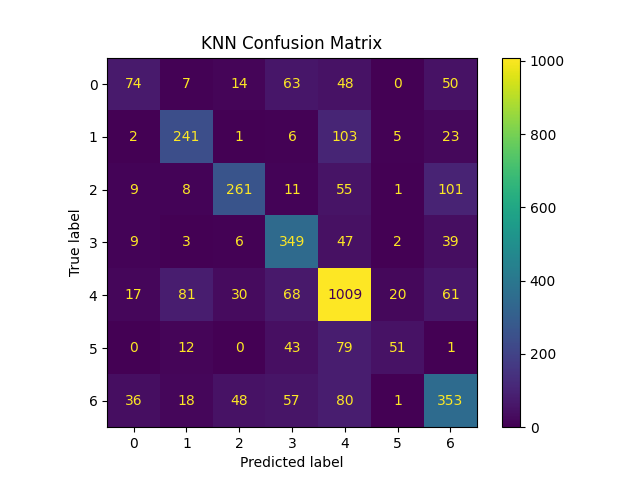
\includegraphics[width=2.5in,height=2in]{images/KNN_Confusion_Matrix.png}
    \captionsetup{font=scriptsize}
    \caption{Confusion matrix for KNN classifier}
    \label{fig:KNN_CM}
\end{figure}

\begin{figure}
    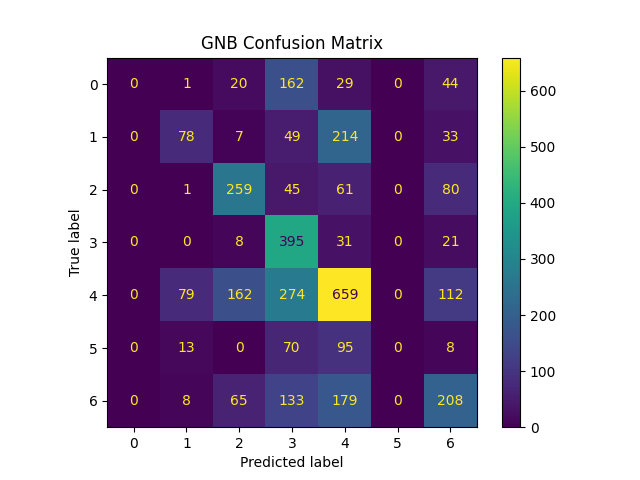
\includegraphics[width=2.5in,height=2in]{images/GNB_Confusion_Matrix.png}
    \captionsetup{font=scriptsize}
    \caption{Confusion matrix for GNB classifier}
    \label{fig:GNB_CM}
\end{figure}

\begin{figure}
    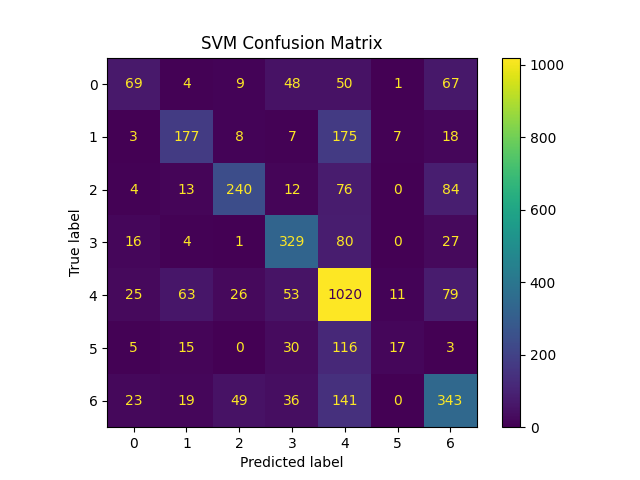
\includegraphics[width=2.5in,height=2in]{images/SVM_Confusion_Matrix.png}
    \captionsetup{font=scriptsize}
    \caption{Confusion matrix for SVM classifier}
    \label{fig:SVM_CM}
\end{figure}

\begin{figure}
    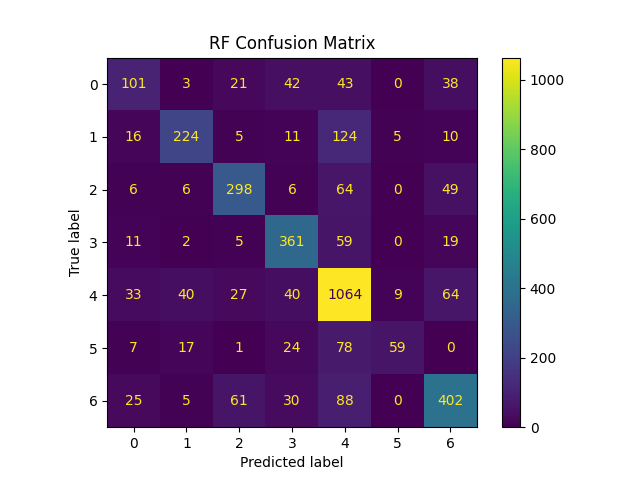
\includegraphics[width=2.5in,height=2in]{images/RF_Confusion_Matrix.png}
    \captionsetup{font=scriptsize}
    \caption{Confusion matrix for Random forest classifier}
    \label{fig:RF_CM}
\end{figure}

\begin{figure}
    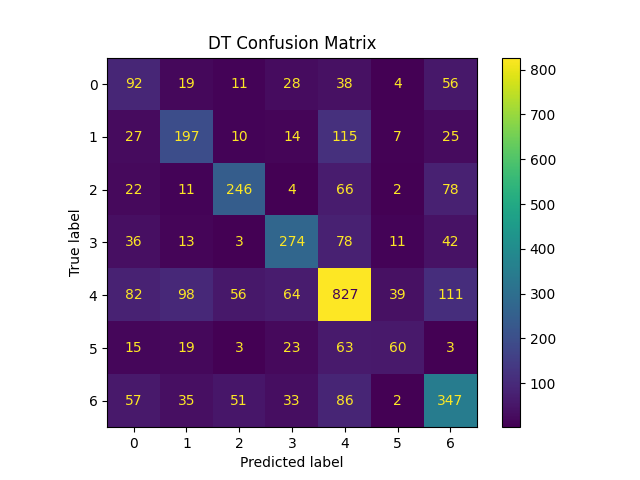
\includegraphics[width=2.5in,height=2in]{images/DT_Confusion_Matrix.png}
    \captionsetup{font=scriptsize}
    \caption{Confusion matrix for Decision tree classifier}
    \label{fig:DT_CM}
\end{figure}

The numbers in the legend show the number of trials for each classifier. This graph shows that, by far, the \textbf{random forest} classifier performs the best with the least variability across all metrics measured. The Gaussian Naive Bayes classifier performed the worst across all metrics measured and also had the greatest variability, most likely due to the feature independence assumption which doesn't hold for our dataset as seen in the correlation matrix given by figure \ref{fig:corr}.

\section{Conclusion}
In conclusion, for the classification problem given of classifying body or car parts in heatmap images, the Random forest classifier performs the most robustly across all metrics measured. It is therefore recommended that the \textbf{random forest} classifier be employed for this and similar image classification problems in disaster scenarios for being able to detect people or people in running cars who might need rescuing, and to most robustly and efficiently differentiate between them and other objects at least 70\% of the time.

% References %
\bibliographystyle{IEEEtran}
% \bibliography{references}

\end{document}